
%% bare_conf.tex
%% V1.3
%% 2007/01/11
%% by Michael Shell
%% See:
%% http://www.michaelshell.org/
%% for current contact information.
%%
%% This is a skeleton file demonstrating the use of IEEEtran.cls
%% (requires IEEEtran.cls version 1.7 or later) with an IEEE conference paper.
%%
%% Support sites:
%% http://www.michaelshell.org/tex/ieeetran/
%% http://www.ctan.org/tex-archive/macros/latex/contrib/IEEEtran/
%% and
%% http://www.ieee.org/

%%*************************************************************************
%% Legal Notice:
%% This code is offered as-is without any warranty either expressed or
%% implied; without even the implied warranty of MERCHANTABILITY or
%% FITNESS FOR A PARTICULAR PURPOSE! 
%% User assumes all risk.
%% In no event shall IEEE or any contributor to this code be liable for
%% any damages or losses, including, but not limited to, incidental,
%% consequential, or any other damages, resulting from the use or misuse
%% of any information contained here.
%%
%% All comments are the opinions of their respective authors and are not
%% necessarily endorsed by the IEEE.
%%
%% This work is distributed under the LaTeX Project Public License (LPPL)
%% ( http://www.latex-project.org/ ) version 1.3, and may be freely used,
%% distributed and modified. A copy of the LPPL, version 1.3, is included
%% in the base LaTeX documentation of all distributions of LaTeX released
%% 2003/12/01 or later.
%% Retain all contribution notices and credits.
%% ** Modified files should be clearly indicated as such, including  **
%% ** renaming them and changing author support contact information. **
%%
%% File list of work: IEEEtran.cls, IEEEtran_HOWTO.pdf, bare_adv.tex,
%%                    bare_conf.tex, bare_jrnl.tex, bare_jrnl_compsoc.tex
%%*************************************************************************

% *** Authors should verify (and, if needed, correct) their LaTeX system  ***
% *** with the testflow diagnostic prior to trusting their LaTeX platform ***
% *** with production work. IEEE's font choices can trigger bugs that do  ***
% *** not appear when using other class files.                            ***
% The testflow support page is at:
% http://www.michaelshell.org/tex/testflow/



% Note that the a4paper option is mainly intended so that authors in
% countries using A4 can easily print to A4 and see how their papers will
% look in print - the typesetting of the document will not typically be
% affected with changes in paper size (but the bottom and side margins will).
% Use the testflow package mentioned above to verify correct handling of
% both paper sizes by the user's LaTeX system.
%
% Also note that the "draftcls" or "draftclsnofoot", not "draft", option
% should be used if it is desired that the figures are to be displayed in
% draft mode.
%
\documentclass[conference]{IEEEtran}
\usepackage{amsmath}
\usepackage{graphicx}
\usepackage{xcolor}
\usepackage{stfloats} % allow full-width figure* at page bottom

% Relax float-placement limits so the pipeline figure and the two bar charts
% pack into the page budget instead of overflowing onto an extra page.
\renewcommand{\topfraction}{0.95}
\renewcommand{\dbltopfraction}{0.95}
\renewcommand{\bottomfraction}{0.7}
\renewcommand{\textfraction}{0.05}
\renewcommand{\floatpagefraction}{0.6}
\renewcommand{\dblfloatpagefraction}{0.6}
\setcounter{topnumber}{3}
\setcounter{dbltopnumber}{3}
\setcounter{bottomnumber}{2}
\setcounter{totalnumber}{5}

% ---------------------------------------------------------------------------
% Figure placeholders.
% These reserve page space for artwork that is still being finalized:
%   - the two evaluation bar charts (fig1_macro_f1_color.png,
%     fig2_ff_per_class_color.png), and
%   - the full-width end-to-end pipeline figure (data collection -> models).
% Drop in the final artwork by replacing the \figplaceholder{...} call with an
% \includegraphics{...} line (the intended file names are noted in each caption).
% ---------------------------------------------------------------------------
\newcommand{\figplaceholder}[3][0.9\linewidth]{%
  \setlength{\fboxsep}{0pt}%
  \fbox{\begin{minipage}[c][#2][c]{#1}%
    \centering
    \color{gray}\itshape
    [\,PLACEHOLDER\,]\\[0.4em]
    #3
  \end{minipage}}%
}
% Add the compsoc option for Computer Society conferences.
%
% If IEEEtran.cls has not been installed into the LaTeX system files,
% manually specify the path to it like:
% \documentclass[conference]{../sty/IEEEtran}





% Some very useful LaTeX packages include:
% (uncomment the ones you want to load)


% *** MISC UTILITY PACKAGES ***
%
%\usepackage{ifpdf}
% Heiko Oberdiek's ifpdf.sty is very useful if you need conditional
% compilation based on whether the output is pdf or dvi.
% usage:
% \ifpdf
%   % pdf code
% \else
%   % dvi code
% \fi
% The latest version of ifpdf.sty can be obtained from:
% http://www.ctan.org/tex-archive/macros/latex/contrib/oberdiek/
% Also, note that IEEEtran.cls V1.7 and later provides a builtin
% \ifCLASSINFOpdf conditional that works the same way.
% When switching from latex to pdflatex and vice-versa, the compiler may
% have to be run twice to clear warning/error messages.






% *** CITATION PACKAGES ***
%
%\usepackage{cite}
% cite.sty was written by Donald Arseneau
% V1.6 and later of IEEEtran pre-defines the format of the cite.sty package
% \cite{} output to follow that of IEEE. Loading the cite package will
% result in citation numbers being automatically sorted and properly
% "compressed/ranged". e.g., [1], [9], [2], [7], [5], [6] without using
% cite.sty will become [1], [2], [5]--[7], [9] using cite.sty. cite.sty's
% \cite will automatically add leading space, if needed. Use cite.sty's
% noadjust option (cite.sty V3.8 and later) if you want to turn this off.
% cite.sty is already installed on most LaTeX systems. Be sure and use
% version 4.0 (2003-05-27) and later if using hyperref.sty. cite.sty does
% not currently provide for hyperlinked citations.
% The latest version can be obtained at:
% http://www.ctan.org/tex-archive/macros/latex/contrib/cite/
% The documentation is contained in the cite.sty file itself.






% *** GRAPHICS RELATED PACKAGES ***
%
\ifCLASSINFOpdf
  % \usepackage[pdftex]{graphicx}
  % declare the path(s) where your graphic files are
  % \graphicspath{{../pdf/}{../jpeg/}}
  % and their extensions so you won't have to specify these with
  % every instance of \includegraphics
  % \DeclareGraphicsExtensions{.pdf,.jpeg,.png}
\else
  % or other class option (dvipsone, dvipdf, if not using dvips). graphicx
  % will default to the driver specified in the system graphics.cfg if no
  % driver is specified.
  % \usepackage[dvips]{graphicx}
  % declare the path(s) where your graphic files are
  % \graphicspath{{../eps/}}
  % and their extensions so you won't have to specify these with
  % every instance of \includegraphics
  % \DeclareGraphicsExtensions{.eps}
\fi
% graphicx was written by David Carlisle and Sebastian Rahtz. It is
% required if you want graphics, photos, etc. graphicx.sty is already
% installed on most LaTeX systems. The latest version and documentation can
% be obtained at: 
% http://www.ctan.org/tex-archive/macros/latex/required/graphics/
% Another good source of documentation is "Using Imported Graphics in
% LaTeX2e" by Keith Reckdahl which can be found as epslatex.ps or
% epslatex.pdf at: http://www.ctan.org/tex-archive/info/
%
% latex, and pdflatex in dvi mode, support graphics in encapsulated
% postscript (.eps) format. pdflatex in pdf mode supports graphics
% in .pdf, .jpeg, .png and .mps (metapost) formats. Users should ensure
% that all non-photo figures use a vector format (.eps, .pdf, .mps) and
% not a bitmapped formats (.jpeg, .png). IEEE frowns on bitmapped formats
% which can result in "jaggedy"/blurry rendering of lines and letters as
% well as large increases in file sizes.
%
% You can find documentation about the pdfTeX application at:
% http://www.tug.org/applications/pdftex





% *** MATH PACKAGES ***
%
%\usepackage[cmex10]{amsmath}
% A popular package from the American Mathematical Society that provides
% many useful and powerful commands for dealing with mathematics. If using
% it, be sure to load this package with the cmex10 option to ensure that
% only type 1 fonts will utilized at all point sizes. Without this option,
% it is possible that some math symbols, particularly those within
% footnotes, will be rendered in bitmap form which will result in a
% document that can not be IEEE Xplore compliant!
%
% Also, note that the amsmath package sets \interdisplaylinepenalty to 10000
% thus preventing page breaks from occurring within multiline equations. Use:
%\interdisplaylinepenalty=2500
% after loading amsmath to restore such page breaks as IEEEtran.cls normally
% does. amsmath.sty is already installed on most LaTeX systems. The latest
% version and documentation can be obtained at:
% http://www.ctan.org/tex-archive/macros/latex/required/amslatex/math/





% *** SPECIALIZED LIST PACKAGES ***
%
%\usepackage{algorithmic}
% algorithmic.sty was written by Peter Williams and Rogerio Brito.
% This package provides an algorithmic environment fo describing algorithms.
% You can use the algorithmic environment in-text or within a figure
% environment to provide for a floating algorithm. Do NOT use the algorithm
% floating environment provided by algorithm.sty (by the same authors) or
% algorithm2e.sty (by Christophe Fiorio) as IEEE does not use dedicated
% algorithm float types and packages that provide these will not provide
% correct IEEE style captions. The latest version and documentation of
% algorithmic.sty can be obtained at:
% http://www.ctan.org/tex-archive/macros/latex/contrib/algorithms/
% There is also a support site at:
% http://algorithms.berlios.de/index.html
% Also of interest may be the (relatively newer and more customizable)
% algorithmicx.sty package by Szasz Janos:
% http://www.ctan.org/tex-archive/macros/latex/contrib/algorithmicx/




% *** ALIGNMENT PACKAGES ***
%
%\usepackage{array}
% Frank Mittelbach's and David Carlisle's array.sty patches and improves
% the standard LaTeX2e array and tabular environments to provide better
% appearance and additional user controls. As the default LaTeX2e table
% generation code is lacking to the point of almost being broken with
% respect to the quality of the end results, all users are strongly
% advised to use an enhanced (at the very least that provided by array.sty)
% set of table tools. array.sty is already installed on most systems. The
% latest version and documentation can be obtained at:
% http://www.ctan.org/tex-archive/macros/latex/required/tools/


%\usepackage{mdwmath}
%\usepackage{mdwtab}
% Also highly recommended is Mark Wooding's extremely powerful MDW tools,
% especially mdwmath.sty and mdwtab.sty which are used to format equations
% and tables, respectively. The MDWtools set is already installed on most
% LaTeX systems. The lastest version and documentation is available at:
% http://www.ctan.org/tex-archive/macros/latex/contrib/mdwtools/


% IEEEtran contains the IEEEeqnarray family of commands that can be used to
% generate multiline equations as well as matrices, tables, etc., of high
% quality.


%\usepackage{eqparbox}
% Also of notable interest is Scott Pakin's eqparbox package for creating
% (automatically sized) equal width boxes - aka "natural width parboxes".
% Available at:
% http://www.ctan.org/tex-archive/macros/latex/contrib/eqparbox/





% *** SUBFIGURE PACKAGES ***
%\usepackage[tight,footnotesize]{subfigure}
% subfigure.sty was written by Steven Douglas Cochran. This package makes it
% easy to put subfigures in your figures. e.g., "Figure 1a and 1b". For IEEE
% work, it is a good idea to load it with the tight package option to reduce
% the amount of white space around the subfigures. subfigure.sty is already
% installed on most LaTeX systems. The latest version and documentation can
% be obtained at:
% http://www.ctan.org/tex-archive/obsolete/macros/latex/contrib/subfigure/
% subfigure.sty has been superceeded by subfig.sty.



%\usepackage[caption=false]{caption}
%\usepackage[font=footnotesize]{subfig}
% subfig.sty, also written by Steven Douglas Cochran, is the modern
% replacement for subfigure.sty. However, subfig.sty requires and
% automatically loads Axel Sommerfeldt's caption.sty which will override
% IEEEtran.cls handling of captions and this will result in nonIEEE style
% figure/table captions. To prevent this problem, be sure and preload
% caption.sty with its "caption=false" package option. This is will preserve
% IEEEtran.cls handing of captions. Version 1.3 (2005/06/28) and later 
% (recommended due to many improvements over 1.2) of subfig.sty supports
% the caption=false option directly:
%\usepackage[caption=false,font=footnotesize]{subfig}
%
% The latest version and documentation can be obtained at:
% http://www.ctan.org/tex-archive/macros/latex/contrib/subfig/
% The latest version and documentation of caption.sty can be obtained at:
% http://www.ctan.org/tex-archive/macros/latex/contrib/caption/




% *** FLOAT PACKAGES ***
%
%\usepackage{fixltx2e}
% fixltx2e, the successor to the earlier fix2col.sty, was written by
% Frank Mittelbach and David Carlisle. This package corrects a few problems
% in the LaTeX2e kernel, the most notable of which is that in current
% LaTeX2e releases, the ordering of single and double column floats is not
% guaranteed to be preserved. Thus, an unpatched LaTeX2e can allow a
% single column figure to be placed prior to an earlier double column
% figure. The latest version and documentation can be found at:
% http://www.ctan.org/tex-archive/macros/latex/base/



%\usepackage{stfloats}
% stfloats.sty was written by Sigitas Tolusis. This package gives LaTeX2e
% the ability to do double column floats at the bottom of the page as well
% as the top. (e.g., "\begin{figure*}[!b]" is not normally possible in
% LaTeX2e). It also provides a command:
%\fnbelowfloat
% to enable the placement of footnotes below bottom floats (the standard
% LaTeX2e kernel puts them above bottom floats). This is an invasive package
% which rewrites many portions of the LaTeX2e float routines. It may not work
% with other packages that modify the LaTeX2e float routines. The latest
% version and documentation can be obtained at:
% http://www.ctan.org/tex-archive/macros/latex/contrib/sttools/
% Documentation is contained in the stfloats.sty comments as well as in the
% presfull.pdf file. Do not use the stfloats baselinefloat ability as IEEE
% does not allow \baselineskip to stretch. Authors submitting work to the
% IEEE should note that IEEE rarely uses double column equations and
% that authors should try to avoid such use. Do not be tempted to use the
% cuted.sty or midfloat.sty packages (also by Sigitas Tolusis) as IEEE does
% not format its papers in such ways.





% *** PDF, URL AND HYPERLINK PACKAGES ***
%
%\usepackage{url}
% url.sty was written by Donald Arseneau. It provides better support for
% handling and breaking URLs. url.sty is already installed on most LaTeX
% systems. The latest version can be obtained at:
% http://www.ctan.org/tex-archive/macros/latex/contrib/misc/
% Read the url.sty source comments for usage information. Basically,
% \url{my_url_here}.





% *** Do not adjust lengths that control margins, column widths, etc. ***
% *** Do not use packages that alter fonts (such as pslatex).         ***
% There should be no need to do such things with IEEEtran.cls V1.6 and later.
% (Unless specifically asked to do so by the journal or conference you plan
% to submit to, of course. )


% correct bad hyphenation here
\hyphenation{op-tical net-works semi-conduc-tor}


\begin{document}
%
% paper title
% can use linebreaks \\ within to get better formatting as desired
\title{Directional Navigability Estimation from Ultra-Low-Resolution Multi-View Thermal Sensing}



\author{Jana Hussien, Faiz Moazam, Gustavo Ramalho, Abdulrahman Al-Taweel, Yaqoob Ansari, and Eduardo Feo-Flushing % <-this % stops a space
\thanks{$^{1}$School of Computer Science, Carnegie Mellon University, {\tt\small \{author1, author2, efeoflus\}@andrew.cmu.edu}, $^{2}$Carnegie Mellon University in Qatar, {\tt\small \{fmaksood\}@andrew.cmu.edu}. %
}}

% conference papers do not typically use \thanks and this command
% is locked out in conference mode. If really needed, such as for
% the acknowledgment of grants, issue a \IEEEoverridecommandlockouts
% after \documentclass

% for over three affiliations, or if they all won't fit within the width
% of the page, use this alternative format:
% 
%\author{\IEEEauthorblockN{Michael Shell\IEEEauthorrefmark{1},
%Homer Simpson\IEEEauthorrefmark{2},
%James Kirk\IEEEauthorrefmark{3}, 
%Montgomery Scott\IEEEauthorrefmark{3} and
%Eldon Tyrell\IEEEauthorrefmark{4}}
%\IEEEauthorblockA{\IEEEauthorrefmark{1}School of Electrical and Computer Engineering\\
%Georgia Institute of Technology,
%Atlanta, Georgia 30332--0250\\ Email: see http://www.michaelshell.org/contact.html}
%\IEEEauthorblockA{\IEEEauthorrefmark{2}Twentieth Century Fox, Springfield, USA\\
%Email: homer@thesimpsons.com}
%\IEEEauthorblockA{\IEEEauthorrefmark{3}Starfleet Academy, San Francisco, California 96678-2391\\
%Telephone: (800) 555--1212, Fax: (888) 555--1212}
%\IEEEauthorblockA{\IEEEauthorrefmark{4}Tyrell Inc., 123 Replicant Street, Los Angeles, California 90210--4321}}




% use for special paper notices
%\IEEEspecialpapernotice{(Invited Paper)}




% make the title area
\maketitle


\begin{abstract}
Reliable perception of navigable indoor spaces remains a challenge for wearable navigation systems, which typically rely on high-resolution cameras, depth sensors, or large annotated datasets---limiting deployability in privacy-sensitive environments and raising development costs.
%
This paper investigates whether directional navigability can be estimated using only ultra-low-resolution thermal imagery from a wearable multi-camera platform, a setting made difficult by the limited detail of low-resolution thermal sensors and the cost of annotating thermal data.
%
We propose a calibration-free learning framework that uses high-resolution RGB imagery during data collection to automatically generate navigability labels, enabling training without manual annotation. The resulting models estimate multi-direction navigability directly from multi-view thermal observations, requiring no geometric calibration, pixel-level alignment, or fixed sensor configuration.
%
Experiments with a wearable rig of three ultra-low-resolution thermal cameras show that directional navigability can be reliably inferred from thermal sensing alone. We further compare multi-camera fusion strategies and evaluate robustness to camera-arrangement changes, highlighting ultra-low-resolution thermal sensing as a scalable, privacy-preserving solution for wearable indoor navigation.


% Reliable perception of navigable indoor spaces remains a fundamental challenge for wearable navigation systems. Existing approaches typically rely on high-resolution RGB cameras, depth sensors, or extensive annotated datasets, limiting their deployability in privacy-sensitive environments and increasing the cost of data collection and model development.
% This paper investigates whether egocentric navigability can be estimated using only ultra-low-resolution thermal imagery captured from a wearable multi-camera platform. Directly training such systems is challenging because ultra-low-resolution thermal sensors provide limited visual detail, multi-camera configurations introduce variability in sensor placement and viewpoints, and obtaining large-scale annotated thermal datasets is costly and labor-intensive.
% To address these challenges, we propose a calibration-free teacher–student learning framework that transfers navigability knowledge from a high-resolution RGB teacher to a wearable thermal student. During data collection, a handheld RGB camera provides training-time supervision by automatically generating navigability labels and soft semantic predictions. The student model learns to estimate navigability directly from temporal sequences of ultra-low-resolution thermal observations captured by multiple cameras. Unlike conventional cross-modal learning approaches, the proposed framework does not require geometric calibration, pixel-level alignment, or a fixed camera arrangement between the teacher and student sensors.
% The proposed approach enables the development of navigation-oriented thermal perception models while substantially reducing annotation effort and deployment constraints. Experimental results demonstrate that teacher-guided training improves navigability estimation performance over models trained solely from hard labels, while maintaining inference using only low-cost thermal sensors. Furthermore, the learned models remain effective across different camera configurations, highlighting the potential of calibration-free knowledge transfer for scalable and privacy-preserving wearable navigation systems.
\end{abstract}
% IEEEtran.cls defaults to using nonbold math in the Abstract.
% This preserves the distinction between vectors and scalars. However,
% if the conference you are submitting to favors bold math in the abstract,
% then you can use LaTeX's standard command \boldmath at the very start
% of the abstract to achieve this. Many IEEE journals/conferences frown on
% math in the abstract anyway.

% no keywords




% For peer review papers, you can put extra information on the cover
% page as needed:
% \ifCLASSOPTIONpeerreview
% \begin{center} \bfseries EDICS Category: 3-BBND \end{center}
% \fi
%
% For peerreview papers, this IEEEtran command inserts a page break and
% creates the second title. It will be ignored for other modes.
\IEEEpeerreviewmaketitle


\section{Introduction}

Wearable navigation aids promise greater independence for visually impaired
users in unfamiliar indoor spaces, but their sensing stacks are costly. Most
rely on high-resolution RGB or active depth sensors, which continuously capture
identifiable imagery of bystanders and raise privacy concerns when worn indoors.
They also require large hand-labeled datasets to learn which directions are
walkable, and typically assume a fixed, geometrically calibrated camera layout
that breaks as soon as a sensor shifts.

Ultra-low-resolution thermal sensing is an appealing alternative. A
$32\times24$-pixel array costs a few tens of dollars, draws little power, is
invariant to lighting, and is too coarse to resolve identifiable facial
features. These same properties make perception hard: each frame carries little
spatial detail, several cameras are needed for useful coverage, and annotating
thermal data is laborious. We therefore ask whether \emph{directional
navigability}---which directions around the wearer are walkable---can be
estimated from ultra-low-resolution thermal imagery alone, without geometric
calibration and without manual labels.

We answer this affirmatively with a calibration-free, RGB-supervised framework
(Fig.~\ref{fig:pipeline}). During data collection only, a high-resolution RGB
camera rides alongside a wearable rig of three ultra-low-resolution thermal
cameras; an off-the-shelf detector run on the RGB frames automatically generates
per-direction navigability labels, so no manual annotation is needed. At
inference the RGB camera is removed: the model consumes only the three raw
thermal tiles and predicts, for each of the left, middle, and right directions,
whether the space is clear, occupied by a person, or blocked by another object.
Because supervision is transferred through labels rather than pixel-aligned
feature matching, the framework needs no calibration, no pixel-level alignment,
and no fixed correspondence between sensor position and input channel.

Within this framework we study two deployment-critical questions---how to fuse
the three views, and how robust the system is to camera placement---which
motivate our contributions: (i)~a calibration-free framework that transfers
navigability supervision from an RGB detector to a thermal-only model, with no
labels or RGB at deployment; (ii)~a direct comparison of three multi-view fusion
strategies (pixel-, decision-, and feature-level) on ultra-low-resolution
thermal data; and (iii)~an analysis showing that a lightweight
camera-identity correction restores accuracy when camera slots are shuffled,
matching a ground-truth oracle re-sort.

\begin{figure*}[!t]
  \centering
  % Replace the placeholder below with the final pipeline artwork, e.g.:
  % \includegraphics[width=\textwidth]{pipeline_overview.png}
  \figplaceholder[\textwidth]{0.15\textheight}{%
    \textbf{Full-width pipeline figure.}\\[0.3em]
    End-to-end overview: wearable three-camera ultra-low-resolution thermal
    capture (RGB camera used only at data-collection time) $\rightarrow$
    RGB/YOLO automatic per-direction label generation $\rightarrow$ the four
    thermal fusion models (stitched panorama, output fusion, feature fusion,
    feature fusion with camera-identity correction) $\rightarrow$ per-direction
    navigability predictions.}
  \caption{End-to-end pipeline, from multi-view thermal data collection and
  RGB-based automatic labeling to the family of thermal fusion models evaluated
  in this paper. The RGB camera is present only during data collection; at
  inference the models use the three ultra-low-resolution thermal tiles alone.}
  \label{fig:pipeline}
\end{figure*}


\section{Related Work}

\subsection{Privacy-Preserving and Ultra-Low-Resolution Thermal Sensing}

Wearable indoor navigation systems for visually impaired users have traditionally relied on RGB cameras or depth sensors, which raises privacy concerns when deployed continuously indoors. Gao~\textit{et al.}'s DareDevil~\cite{gao2025daredevil} addresses this by auto-labeling thermal frames from a paired RGB camera through a pretrained YOLOv8 detector, avoiding manual annotation. However, DareDevil collapses all object classes into a single binary obstacle label and operates on colorized thermal frames from a single standard-resolution thermal camera at inference time; it does not address the extreme spatial compression of a $32\times24$-pixel array, multi-camera fusion, or robustness to sensor placement.

A separate line of work uses ultra-low-resolution thermal sensors (e.g., $24\times32$ arrays, on the order of \$30 per unit) as a low-power, lighting-invariant alternative to RGB and depth sensing. Such sensors are too coarse to resolve identifiable facial features, but their reduced spatial detail also degrades the features downstream perception models rely on; prior work compensates for this by fusing thermal imagery with gyroscope readings for motion estimation~\cite{thermal_gyro_odom}. Naser~\textit{et al.}~\cite{naser2022calibration} separately showed that most low-resolution thermal pipelines still assume a fixed, calibrated sensor geometry. This work targets discrete navigability classification rather than continuous odometry, and removes the dependence on geometric calibration that these systems retain.

\subsection{Automatic Label Generation for Traversability}

Manually annotating walkable regions is expensive and does not scale to real-world indoor environments. Kim~\textit{et al.}~\cite{kim2024traversability} addressed this for egocentric video with an automated annotation strategy that derives traversability labels without manual pixel-level annotation. We apply this same philosophy to a cross-modal setting: RGB-derived object detections supervise a thermal-only model only during data collection, and the RGB sensor is entirely absent at deployment.

\subsection{Large-Scale and Web-Sourced Navigation Learning}

CityWalker~\cite{liu2025citywalker} trains an embodied urban navigation policy on over 2{,}000 hours of in-the-wild web video, using visual odometry to generate pseudo-labels instead of teleoperated demonstrations. CityWalker targets continuous waypoint-following from RGB video; this work targets discrete per-direction navigability from privacy-preserving thermal sensing, with an order of magnitude less data collected from a purpose-built wearable rig.

\subsection{Multi-View Sensor Fusion and Placement Robustness}

Multi-camera perception systems typically assume a fixed mapping between physical sensor position and input channel, an assumption that breaks when sensors shift or are reattached in a different order on a wearable rig. Pixel-level, decision-level, and feature-level fusion are well studied in the sensor fusion literature, but little work examines how these strategies behave when the camera-to-slot assignment is perturbed, particularly at the small camera counts and extreme resolutions considered here. This also relates to cross-resolution knowledge transfer, where a high-resolution signal supervises a model on coarser inputs~\cite{qi2021msad}; our gap is larger still, since the supervisory RGB detector and the deployed $32\times24$ thermal arrays share no feature space and no geometric alignment at inference time. We contribute a direct comparison of three fusion strategies for an ultra-low-resolution, three-camera array, together with an explicit treatment of camera-slot permutation robustness.


\section{Methodology}


\subsection{Problem Formulation}
% Input:

% Three thermal images.
% Output:
% Left, Front, Right navigability states.

\subsection{RGB-Based Automatic Label Generation}
% RGB frame
%  YOLO detections
%  spatial post-processing
%  left/front/right navigability labels.

% Explain:

% image partitioning,
% occupancy rules,
% label generation.

\subsection{Thermal Fusion Architectures}

We evaluate four architectures for estimating per-direction navigability from the three active thermal cameras (left, middle, right), each consuming only raw $32\times24$ thermal tiles at inference time and producing a 3-class prediction per camera over $\{\texttt{no\_object}, \texttt{person}, \texttt{other\_object}\}$. The four span pixel-level, decision-level, and feature-level fusion, plus a fourth variant that adds a learned correction for camera-placement permutations on top of feature-level fusion. All but the stitched-panorama baseline share a configurable convolutional backbone, \texttt{FlexBackbone} (depth $d \in \{2,\dots,5\}$, width multiplier $w$, activation $a \in \{\text{ReLU}, \text{GELU}, \text{LeakyReLU}\}$), which returns the intermediate feature map at every block so downstream heads can pool over multiple resolutions.

\paragraph{Model 1: Stitched Panorama (pixel-level fusion)} The three raw tiles are warped into a shared panoramic canvas via pre-computed thermal-to-thermal homographies, producing a two-channel panorama (raw intensity plus a validity mask). A fixed five-layer backbone is applied independently to each camera's bounding-box crop of the panorama, followed by a shared classification head. Because the panorama is built once, before any learned processing, cross-camera information lost to the homography warp is unavailable to the model; this baseline isolates the cost of fusing at the pixel level.

\paragraph{Model 2: Output Fusion (decision-level fusion)} A shared-weight \texttt{FlexBackbone} processes each camera's tile independently, and a per-camera head reduces it to one 3-class logit vector. The three logit vectors are concatenated and passed through a small fusion MLP that refines them jointly. Fusion only ever sees already-classified, low-dimensional logits, so cross-camera interaction is limited to statistical dependencies between directions rather than raw spatial features.

\paragraph{Model 3: Feature Fusion} The same shared-weight backbone runs on each camera's tile, but instead of classifying each camera separately, the feature maps from all three cameras at a given backbone level are concatenated channel-wise and projected back to the original channel count via a learned $1\times1$ convolution, applied at every level. This yields a single fused multi-scale feature pyramid mixing all three cameras at every depth, in contrast to Model 2's late fusion. A shared head then produces the final per-camera logits. We sweep backbone depth, width, activation, and head capacity to select the configuration used as the reference Feature Fusion result throughout this paper.

\paragraph{Model 4: Feature Fusion with camera-identity correction} Model 3's per-level $1\times1$ projections consume all cameras' features in a fixed slot order, so the projection layer can learn to associate an input slot with a physical direction even though the backbone itself is fully shared and permutation-agnostic; if a sensor is reattached in a different slot at deployment time, this learned positional dependence can degrade predictions. We correct for it with a lightweight auxiliary \texttt{CameraIdentityClassifier}, a compact CNN that takes one raw thermal tile and predicts a 3-way softmax over $\{\text{left}, \text{middle}, \text{right}\}$, trained independently using the true camera-to-direction mapping recorded at capture time. At inference, given a possibly shuffled set of tiles, the classifier scores every slot against every direction and picks the assignment that maximizes total log-probability, enumerated exhaustively over all $3! = 6$ permutations; the resorted tiles are then passed to the unmodified Model 3. We compare this against an oracle re-sort using ground-truth identities (an upper bound on achievable robustness) and a blind condition with no correction at all.

All four architectures share the same masked, per-camera, three-class cross-entropy training objective, gated by a per-camera validity mask so that timesteps without a labeled RGB frame do not contribute gradient.

\section{Experimental Setup}


\subsection{Wearable Thermal Data Collection Platform}

%Paragraph 1 — Overview and Motivation
%Introduce the device and design goals.
We developed a wearable thermal sensing platform designed for privacy-preserving indoor navigation research. The platform consists of multiple ultra-low-resolution thermal cameras mounted on a wearable frame and connected to an embedded computing unit for synchronized data acquisition. The design emphasizes low cost, privacy preservation, and flexibility, making it suitable for studying navigation perception under severe sensing constraints.


%Paragraph 2 — Hardware Description
%Describe the hardware without excessive detail.

The wearable platform incorporates multiple MLX90640 SparkFun IR Array Breakout sensors, each providing a $32\times24$ thermal image of the environment. The sensors are mounted at different viewing angles to increase environmental coverage and capture complementary observations of the user's surroundings. All sensors are connected to an NVIDIA Jetson Nano-based acquisition unit that records timestamped thermal frames for subsequent processing.

% Paragraph 3 — Data Collection Procedure
% Explain how data are acquired.



\subsection{Data Collection}

Data were recorded by walking the wearable rig through indoor environments while
a high-resolution RGB camera, rigidly mounted alongside the thermal array,
captured a time-synchronized reference stream used only for label generation.
During each traversal the three active thermal cameras and the RGB camera
recorded timestamped frames continuously, producing sequences that span clear
corridors as well as encounters with people and static objects, so that all
three navigability states are represented across the left, middle, and right
directions. Only the thermal tiles and their automatically generated
per-direction labels (Section~\ref{sec:labels}) are retained for model training;
the RGB stream is discarded after labeling and is never available at inference.

\subsection{Training Protocol}

To avoid leaking temporally adjacent, near-duplicate frames across splits, we use
a blocked partition: each recording is divided into contiguous blocks and the
final $20\%$ of every block is held out for validation, giving a train/validation
split that keeps correlated neighbors together. Camera-identity-shuffle
experiments are additionally evaluated on a held-out test set. All learned models
share the same masked, per-camera, three-class cross-entropy objective and are
trained with Adam (learning rate $10^{-3}$, weight decay $10^{-4}$) under a
cosine-annealing schedule for $30$ epochs at batch size $64$, with class
weighting to counter the imbalance toward clear directions. For Feature Fusion we
additionally sweep backbone depth, width, activation, and head capacity and
report the best configuration. We evaluate with per-class $F_1$ score reported
per direction (left, middle, right) and overall; because the label distribution
is skewed toward clear directions, macro-averaged $F_1$ is used for model
selection rather than raw accuracy.

\section{Results}

\begin{figure*}[!t]
  \centering
  % Replace with the final bar chart (native aspect ratio approx 2.8:1):
  % 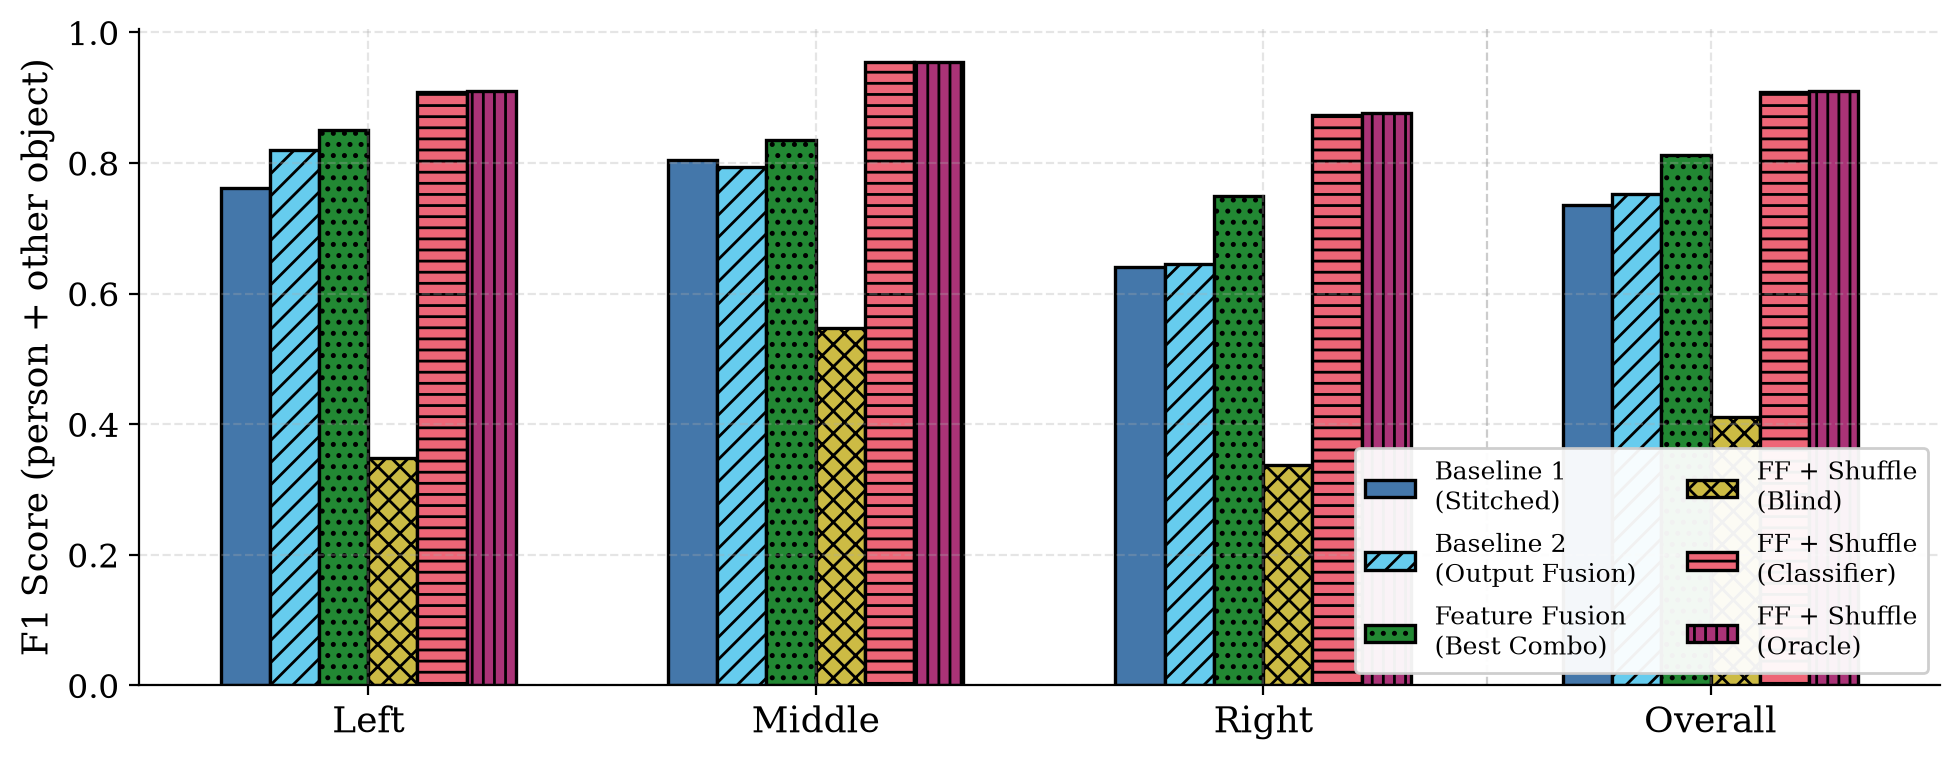
\includegraphics[width=\textwidth]{fig1_macro_f1_color.png}
  \figplaceholder[\textwidth]{0.13\textheight}{%
    \textbf{Bar chart 1: architecture comparison.}\\[0.3em]
    Per-class $F_1$ by camera direction for the four architectures
    (\texttt{fig1\_macro\_f1\_color.png}).}
  \caption{Per-class $F_1$ by camera direction for the obstruction-detection
  architectures. Baselines and Feature Fusion are evaluated on the validation
  set; Feature Fusion with shuffle correction (blind, classifier, oracle) is
  evaluated on the held-out test set.}
  \label{fig:arch_f1}
\end{figure*}

\subsection{Navigability Estimation Performance}

Figure~\ref{fig:arch_f1} compares the four architectures using per-class $F_1$
broken down by camera direction. All models estimate the three navigability
states well above chance from the raw $32\times24$ thermal tiles, confirming that
directional navigability is recoverable from ultra-low-resolution thermal sensing
alone. On the validation set, Feature Fusion is the strongest of the calibrated
(non-shuffled) models, reaching overall per-class $F_1$ of roughly $0.81$
(clear), $0.83$ (person), and $0.80$ (other object). The stitched-panorama and
output-fusion baselines trail it, with overall $F_1$ near $0.73$--$0.78$, and
both show markedly weaker person detection on the right camera, where the useful
thermal signal is sparsest.

\subsection{Fusion Strategy Analysis}

Feature-level fusion consistently outperforms both pixel-level stitching and
decision-level output fusion. Mixing intermediate feature maps across cameras at
every backbone depth preserves cross-camera spatial detail that the alternatives
discard: the stitched panorama warps and blurs the already-coarse thermal signal
before the model sees it, while output fusion only combines low-dimensional,
already-classified logits. Feature fusion costs extra backbone passes, but on
these ultra-low-resolution tiles the accuracy gain justifies the compute, so we
adopt it as the reference architecture for the robustness study.

\begin{figure}[!b]
  \centering
  % Replace with the final bar chart (native aspect ratio approx 1.75:1):
  % 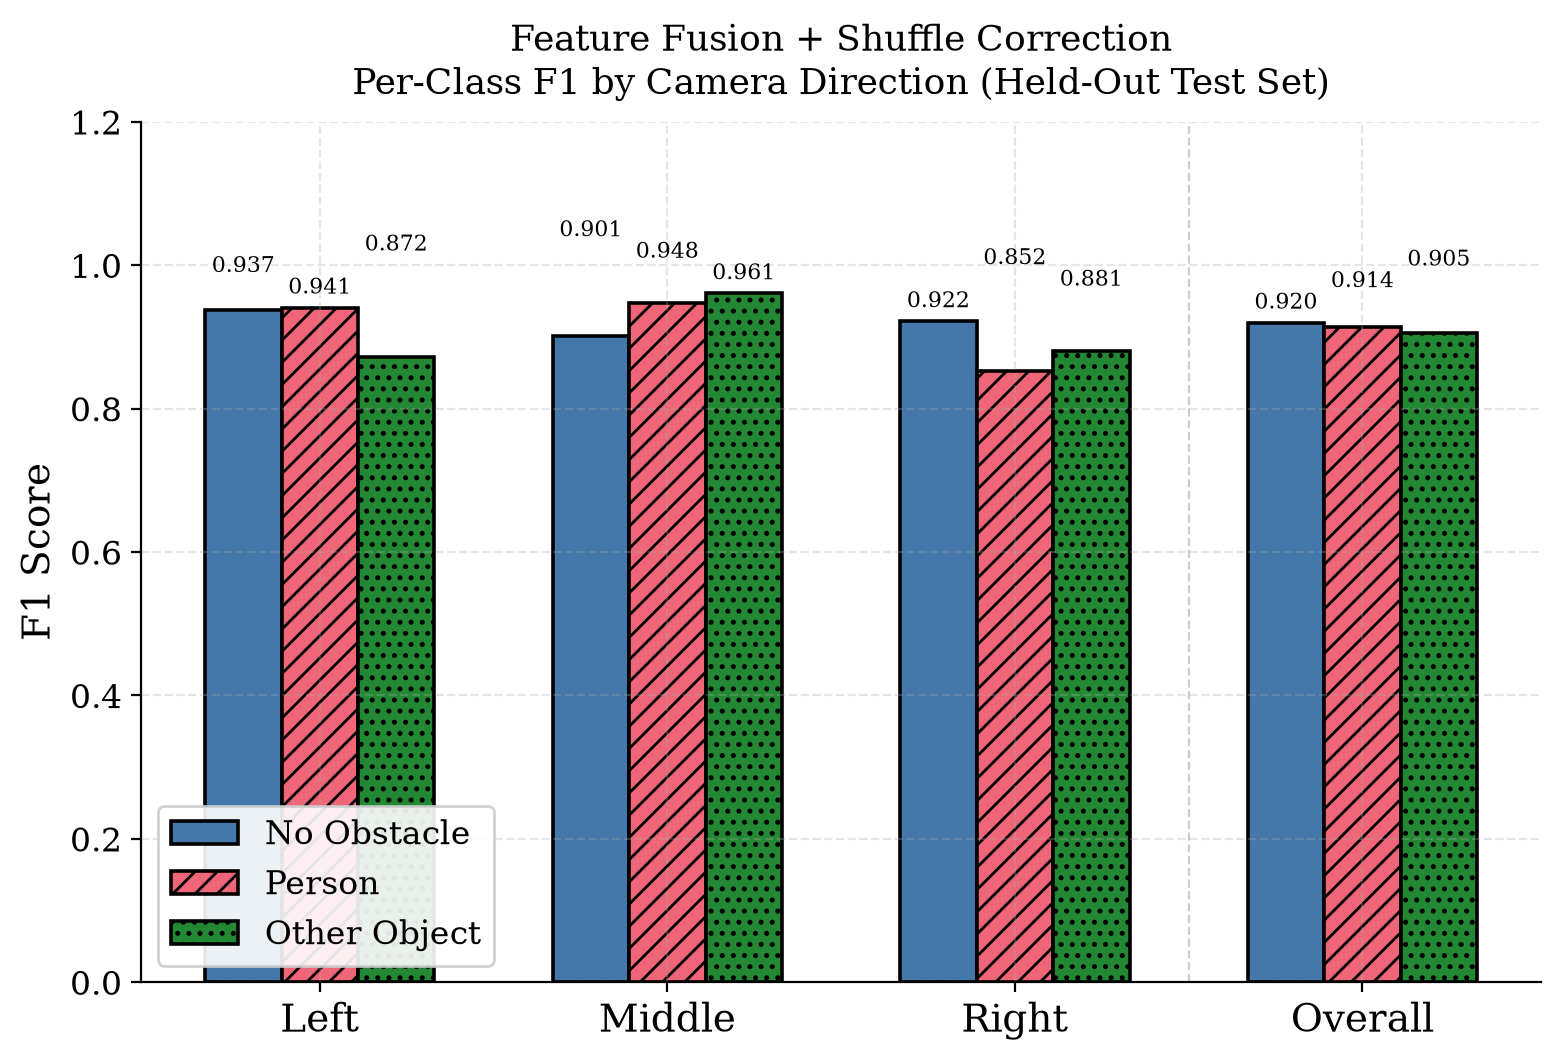
\includegraphics[width=\linewidth]{fig2_ff_per_class_color.png}
  \figplaceholder[\linewidth]{0.11\textheight}{%
    \textbf{Bar chart 2: shuffle-corrected Feature Fusion.}\\[0.3em]
    Per-class $F_1$ by direction and overall
    (\texttt{fig2\_ff\_per\_class\_color.png}).}
  \caption{Per-class $F_1$ of Feature Fusion with classifier-based shuffle
  correction on the held-out test set, broken down by camera direction (left,
  middle, right) and overall.}
  \label{fig:ff_shuffle}
\end{figure}

\subsection{Camera Arrangement Robustness}

Figure~\ref{fig:ff_shuffle} reports Feature Fusion under permuted camera slots on
the held-out test set. Without correction (blind), shuffling the physical
camera-to-slot assignment collapses performance to overall per-class $F_1$ near
$0.40$--$0.42$, confirming that the fixed-slot projection layers learn a
positional dependence that does not survive re-arrangement. The lightweight
camera-identity classifier, which re-sorts tiles to their most likely directions
before the unmodified model, restores overall $F_1$ to roughly $0.90$--$0.92$
across all three classes---matching the ground-truth oracle re-sort to within
rounding. Once tiles are routed to the correct directions the underlying features
are themselves directionally meaningful, so the system is robust to camera
placement rather than overfit to which camera feeds which input channel.


% conference papers do not normally have an appendix


% use section* for acknowledgement
\section*{Acknowledgment}


The authors would like to thank...





% trigger a \newpage just before the given reference
% number - used to balance the columns on the last page
% adjust value as needed - may need to be readjusted if
% the document is modified later
%\IEEEtriggeratref{8}
% The "triggered" command can be changed if desired:
%\IEEEtriggercmd{\enlargethispage{-5in}}

% references section

% can use a bibliography generated by BibTeX as a .bbl file
% BibTeX documentation can be easily obtained at:
% http://www.ctan.org/tex-archive/biblio/bibtex/contrib/doc/
% The IEEEtran BibTeX style support page is at:
% http://www.michaelshell.org/tex/ieeetran/bibtex/
%\bibliographystyle{IEEEtran}
% argument is your BibTeX string definitions and bibliography database(s)
%\bibliography{IEEEabrv,../bib/paper}
%
% <OR> manually copy in the resultant .bbl file
% set second argument of \begin to the number of references
% (used to reserve space for the reference number labels box)
\begin{thebibliography}{6}

\bibitem{gao2025daredevil}
J.~Gao, H.~K. Gedawy, E.~Feo-Flushing, and K.~A. Harras, ``A Deployable
  Privacy-Preserving Thermal-Based Obstacle Detection System for Indoor
  Navigation (DareDevil),'' in \emph{Proc. IEEE ICC}, 2025.

\bibitem{kim2024traversability}
Y.~Kim, J.~H. Lee, C.~Lee, \emph{et al.}, ``Learning Semantic
  Traversability With Egocentric Video and Automated Annotation
  Strategy,'' \emph{IEEE Robotics and Automation Letters}, vol.~9, no.~11,
  pp.~10423--10430, 2024.

\bibitem{liu2025citywalker}
X.~Liu, J.~Li, Y.~Jiang, \emph{et al.}, ``CityWalker: Learning Embodied
  Urban Navigation from Web-Scale Videos,'' in \emph{Proc. CVPR}, 2025.

\bibitem{naser2022calibration}
A.~Naser, A.~Lotfi, and J.~Zhong, ``Calibration of Low-Resolution Thermal
  Imaging for Human Monitoring Applications,'' \emph{IEEE Sensors
  Letters}, vol.~6, no.~3, pp.~1--4, 2022.

\bibitem{thermal_gyro_odom}
% TODO(authors): replace with the full citation for the ultra-low-resolution
% thermal-gyro odometry paper referenced in Section II-A.
Authors, ``Title,'' \emph{Venue}, year. [citation needed]

\bibitem{qi2021msad}
% TODO(authors): replace with the full citation for the multi-scale aligned
% distillation (MSAD) paper referenced in Section II-D.
Authors, ``Title,'' \emph{Venue}, year. [citation needed]

\end{thebibliography}




% that's all folks
\end{document}

